% latex main
% dvips -Pprosper -o main.ps main.dvi
% ps2pdf main.ps main.pdf
\documentclass[pdf,nototal,myframes,slideColor,colorBG]{prosper}

\usepackage{pstricks,pst-node,pst-text,pst-3d}
\usepackage[utf8]{inputenc}
\usepackage{amsmath}


\usepackage{graphicx,color,latexsym}

\newenvironment{cslide}[1]{\begin{slide}{\blue #1}}{\end{slide}}
\newcommand{\emcolorbox}[1]{\colorbox{yellow}{#1}}

\slideCaption{}

\begin{document}

\title{Isabelle/HOL --- A Practical Introduction}
\author{Tobias Nipkow
\\{\small joint work with Larry Paulson and Markus Wenzel}
}
\institution{Technische Universität München
\\ \vspace{0.5cm}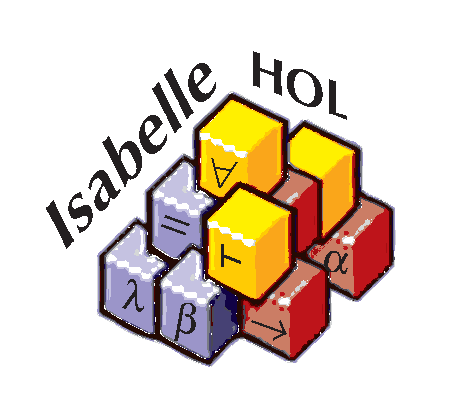
\includegraphics[scale=.4]{isabelle_hol}
}
\maketitle

%-----------------------------------------------------------------------------
\begin{cslide}{What is {\blue Isabelle}?}
\begin{itemize}
\item A \emph{logical framwork}
\item A generic theorem prover
\item A system for implementing proof assistants
\end{itemize}
\end{cslide}
%-----------------------------------------------------------------------------
\overlays{5}{
\begin{cslide}{What is {\blue Isabelle/HOL}?}
\FromSlide{2}
\begin{itemize}
\item An interactive proof assistant
\FromSlide{3}
\item {\small for higher-order logic}
\FromSlide{4}
\item Similar to HOL, PVS, Coq, \dots
\FromSlide{5}
\item But different enough (e.g. \emph{structured proofs})
\end{itemize}
\end{cslide}}
%-----------------------------------------------------------------------------
\overlays{2}{
\begin{cslide}{Why Theorem Proving/Verification/\dots?}
\FromSlide{2}
\vfill
\begin{center}
\Large \emph{\red Because!}
\end{center}
\vfill
\end{cslide}}
%-----------------------------------------------------------------------------
\overlays{2}{
\begin{cslide}{Overview of course}
\begin{enumerate}
\item Introduction to Isabelle/HOL (LNCS 2283)
\begin{itemize}
\item Definitions (datatypes, functions, relations, \dots)
\item Proofs (tactic style)
\end{itemize}
\FromSlide{2}
\item Structured proofs (\emph{Isar})
\end{enumerate}
\end{cslide}}
%-----------------------------------------------------------------------------
\overlays{2}{
\begin{cslide}{Proof styles}
\begin{tabular}{cc}
\begin{tabular}{l}
\texttt{apply(induct\_tac $x$)}\\
\texttt{apply simp}\\
\texttt{apply(rule allI)+}\\
\texttt{apply assumption}\\
\vdots
\end{tabular}
&
\FromSlide{2}
\begin{tabular}{l}
\texttt{proof (induct $x$)}\\
\quad \texttt{show $P(0)$ by simp}\\
\texttt{next}\\
\quad \texttt{assume $P(n)$}\\
\quad \texttt{hence $Q$  by simp}\\
\quad \texttt{thus $P(n+1)$  by blast}\\
\texttt{qed}
\end{tabular}\\\\
Tactic style & \FromSlide{2} Structured (Mizar, Isar)
\end{tabular}
\end{cslide}}
%-----------------------------------------------------------------------------
\begin{cslide}{}
\vfill
\begin{center}
\Large Part 1\\[2em]
Introduction to Isabelle/HOL
\end{center}
\end{cslide}
%-----------------------------------------------------------------------------
\begin{cslide}{Overview of Part 1}
\begin{itemize}
\item Functional Programming
\item Logic
\item Sets and Relations
\end{itemize}
\end{cslide}
%-----------------------------------------------------------------------------
\overlays{2}{
\begin{cslide}{Functional Programming}
\begin{itemize}
\item An introductory example
\item Proof by simplification
\item Case study: Expression compiler
\item Advanced datatypes
\item Advanced recursive functions
\end{itemize}
\FromSlide{2}
There is more:\\
\emph{\blue records},
\emph{\blue (axiomatic) type classes},
\emph{\blue program extraction}, \dots!
\end{cslide}}
%-----------------------------------------------------------------------------
\begin{cslide}{Logic (Natural Deduction)}
\begin{itemize}
\item Propositional logic
\item Quantifiers
\item Automation
\item Forward proof
\end{itemize}
\end{cslide}
%-----------------------------------------------------------------------------
\begin{cslide}{Sets and Relations}
\begin{itemize}
\item Introduction to the library
\item Case study: verified model checking
\item Inductively defined sets
\end{itemize}
\end{cslide}
%-----------------------------------------------------------------------------
\begin{cslide}{}
\vfill
\begin{center}
\Large Part 2\\[2em]
Structured Proofs in Isabelle/Isar/HOL
\end{center}
\end{cslide}
%-----------------------------------------------------------------------------
\begin{cslide}{Motto}
\vfill
\begin{center}
\Large\emcolorbox{Proofs should be readable}
\end{center}
\end{cslide}
%-----------------------------------------------------------------------------
\begin{cslide}{Why Readable Proofs?}
\begin{itemize}
\item Communication
\item Maintenance
\end{itemize}
\end{cslide}
%-----------------------------------------------------------------------------
\overlays{2}{
\begin{cslide}{A Proof Skeleton}
\begin{tabular}{l}
\textbf{proof}\\
\quad\textbf{assume} {\blue\sl assumption}\\
\quad\textbf{have} {\blue\sl intermediate result} \textbf{by} ...\\
\quad\vdots\\
\quad\textbf{have} {\blue\sl intermediate result} \textbf{by} ...\\
\quad\textbf{show} {\blue\sl conclusion} \textbf{by} ...\\
\textbf{qed}
\end{tabular}
\bigskip

\FromSlide{2}
Proves {\blue\sl assumption $\Longrightarrow$ conclusion}
\end{cslide}}
%-----------------------------------------------------------------------------
\overlays{2}{
\begin{cslide}{Proofs and Statements}
\begin{center}
\begin{tabular}{@{}lrl@{}}
\emph{proof} & ::= & \textbf{proof} \emph{statement}* \textbf{qed} \\
                 &$\mid$& \textbf{by} \emph{method}\\[2ex]
\FromSlide{2}
\emph{statement} &\FromSlide{2}::= & \FromSlide{2}\textbf{assume} \emph{propositions} \\
             &\FromSlide{2}$\mid$& \FromSlide{2}(\textbf{show} $\mid$ \textbf{have})
                      \emph{proposition} \emph{proof}
\end{tabular}
\end{center}
\end{cslide}}
%-----------------------------------------------------------------------------
\begin{cslide}{Overview of Part 2}
\begin{itemize}
\item Logic
\item Induction
\item Calculation
\end{itemize}
\end{cslide}
%-----------------------------------------------------------------------------

\end{document}

%%% Local Variables: 
%%% mode: latex
%%% TeX-master: t
%%% End: 
